


\documentclass[11pt,landscape]{report}
\usepackage{graphicx}
\usepackage{amssymb}
\usepackage[colorlinks]{hyperref}

\newcommand{\SupNum}{5}
\textwidth = 10 in
\textheight = 7.0 in
\oddsidemargin = -0.5 in
\evensidemargin = -0.5 in
\topmargin = -0.5 in
\headheight = 0.0 in
\headsep = 0.0 in
\footskip = 0.65 in
\parskip = 0.2in
\parindent = 0.0in


\makeatletter
\renewcommand{\thefigure}{\ifnum \c@chapter>\z@ \thechapter.\fi S\SupNum{}--\@arabic\c@figure}
\renewcommand*\l@figure{\@dottedtocline{1}{1.5em}{3.3em}}
\renewcommand{\thesection}{}
\renewcommand\section{\@startsection {section}{1}{-5.6mm}%
                                   {-3.5ex \@plus -1ex \@minus -.2ex}%
                                   {2.3ex \@plus.2ex}%
                                   {\normalfont\Large\bfseries}}

\makeatother


\newcommand{\ArticleName}{``An Assessment of Sibship Reconstruction \\
Programs with Simulated Microsatellite Data''}

\author{Eric C. Anderson\thanks{\em Fisheries Ecology Division, Southwest Fisheries Science Center, National Marine Fisheries Service, NOAA, Santa Cruz, CA} \and 
Anthony Almudevar\thanks{{\em Department of Biostatistics and Computational Biology,University of Rochester Medical School, Rochester, NY}}
}



\newcommand{\nosibs}{{NoSibs}}
\newcommand{\allhalf}{{AllHalf}}
\newcommand{\allpathalf}{{AllPatHalf}}
\newcommand{\sfsnoh}{{SmallSGs}}
\newcommand{\sfswh}{{SmallSGs\_H}}
\newcommand{\slfsgnoh}{{BigSGs}}
\newcommand{\slfsgwh}{{BigSGs\_H}}
\newcommand{\onelargenoh}{{OneBig}}
\newcommand{\onelargewh}{{OneBig\_H}}
\newcommand{\lottalarge}{{LottaLarge}}

\newcommand{\PD}{\mathrm{PD}}
\newcommand{\PDT}{\mathrm{PD^T}}
\newcommand{\PDS}{\mathrm{PD_S}}
\newcommand{\PDST}{\mathrm{PD_S^T}}
\newcommand{\W}{\mathrm{PD_{AP}}} % W for wrong! = PD from assignment problem on a set cover
\newcommand{\WT}{\mathrm{PD_{AP}^T}}
\newcommand{\FIG}{Figure}

\newcommand{\colony}{{\sc colony}}
\newcommand{\prt}{{\sc prt}}
\newcommand{\kinalyzer}{{\sc kinalyzer}}
\newcommand{\familyfinder}{{\sc familyfinder}}


\title{Supplement \SupNum{} to Article:\\
\ArticleName\\
\mbox{}\\
{\em Running Times of Programs}}



\begin{document}
\maketitle
\section{Overview/Orientation}
This supplement contains plots of the running times of each of the programs. \kinalyzer{} does not appear here because in many cases it required run times that were considerably higher than the other programs and including them on the plot obscured the differences between other methods. 
Running times are presented as boxplots with dot-strips next to them.  There are a few special features of the plots used to prevent the $y$-axis from being too expansive due to outliers.   All of those features are shown in this example figure: 
\begin{center}
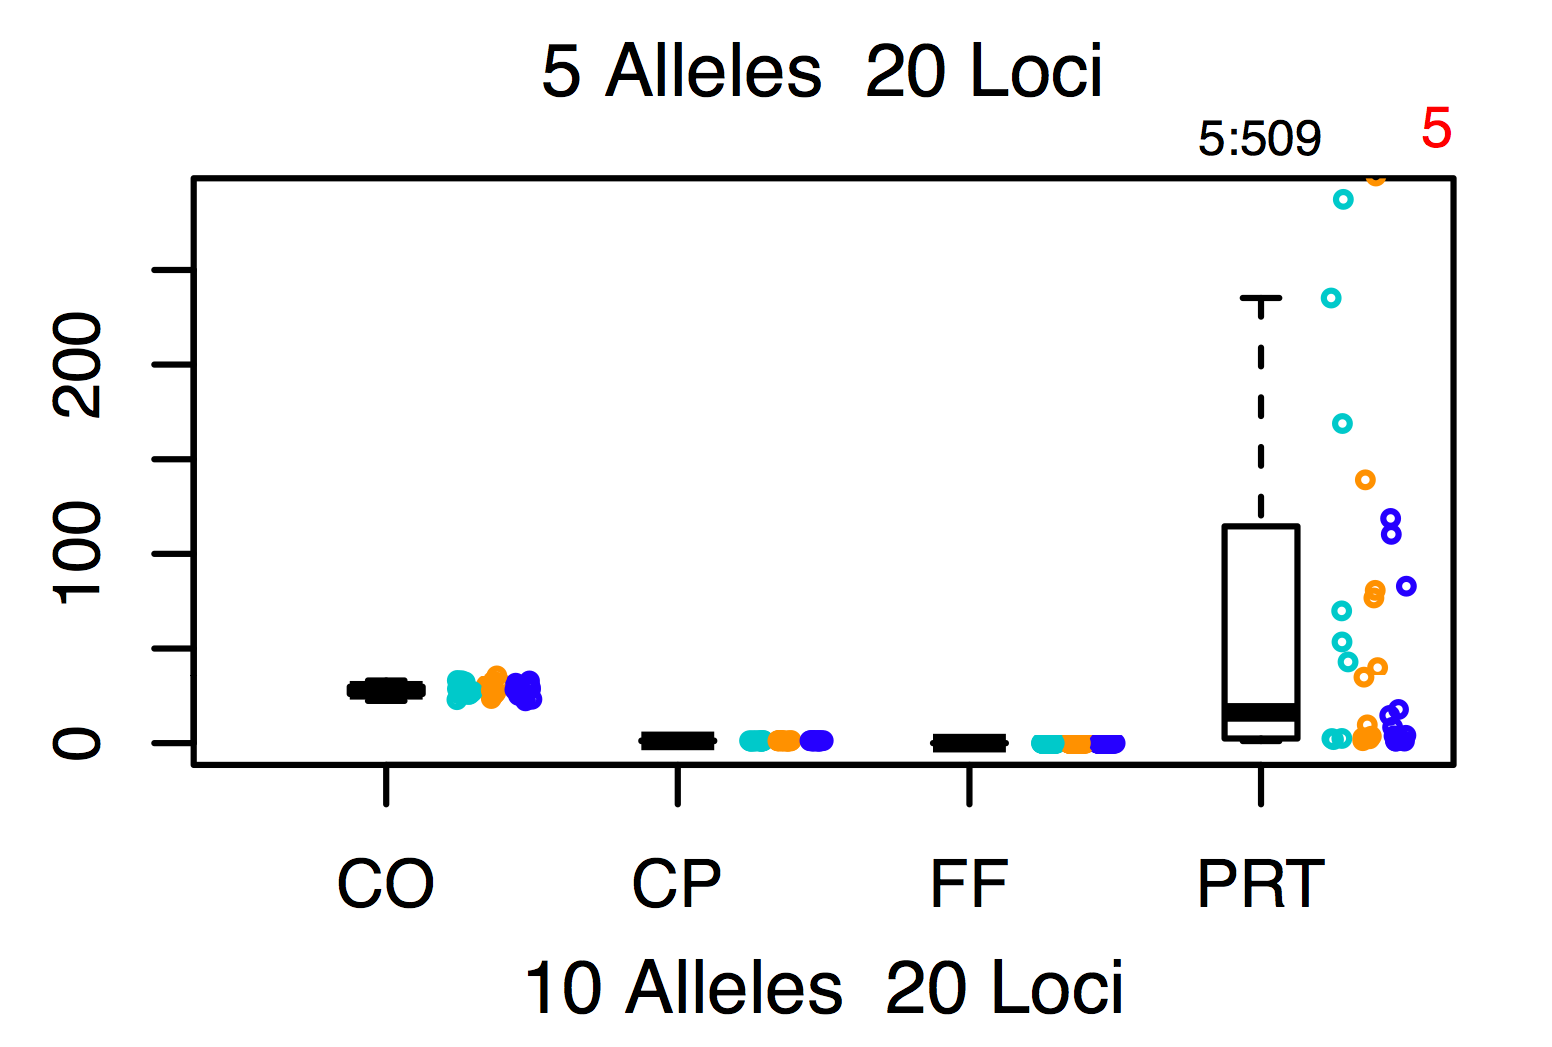
\includegraphics[width=.4\textwidth]{suppl4_example_noki.png}
\end{center}
Running time is presented in minutes on the $y$ axis of every plot.  Extreme outliers that would make the upper limit of the $y$ axis too high were excluded from the plots.  However the occurrence of such outliers for each method is recorded: if there were $N$ outliers for a method and the mean of those outliers was $\mu$ then there is an annotation of the form  ``$N$:$\mu$'' on the top margin of the plot above the boxplot.  In the above example, \prt{}'s boxplot excludes 5 outliers whose mean was 509 minutes.

Additionally, on some data sets, \prt{} did not finish in a reasonable time and was terminated.  The number of such occurrences for each plot panel (if any) is indicated by the red numeral at the top right of the plot.  In the example, that number is 5.

Individual points for running times with data having the different genotyping error rates appear in the dot strips to the right of the boxplots.  Going left to right, dark turquoise =  no error, orange = $d=0.02$, $m=0.01$, and blue = $d=0.07$, $m=0.03$.


For the $n75$ scenarios, boxplots are based on sample sizes of 45 for \prt{}, \colony{}, and \colony{}-P (15 replicates at each of 3 genotyping error rates),  and sample sizes of 150 for Family Finder (50 reps at each of three different rates of genotyping error).  For the \lottalarge{} scenarios, results are based on sample sizes of 15 (5 replicates at 3 genotyping error rates) for \colony{} and \colony-P{}, sizes of 45 for \prt{} (15 replicates at 3 genotyping error rates) and, as with the $n75$ data sets, a sample size of 150 for \familyfinder{}. 

 
Boxplots for \colony{} and \colony{}-P count time in real time, while the results for \prt and \familyfinder count time in user time.  However, since \colony was always run on a dedicated processor, these times are directly comparable.
\newpage

\tableofcontents

\listoffigures

\part{Plots comparing \colony{}, \colony{}-P, \familyfinder{}, and \prt}

\input{../../tmp/plots/running_times/running_times_latex_include.tex}

\end{document}